\PassOptionsToPackage{numbers,sort&compress}{natbib}
\documentclass[preprint,numbers,a4paper]{elsarticle}
\usepackage[T1]{fontenc}
\usepackage[utf8]{inputenc}
\usepackage{amsmath,amssymb,bm,booktabs,graphicx,siunitx}
\usepackage[margin=2cm]{geometry}
\usepackage{hyperref}
\graphicspath{{figures/}}
\usepackage{xr-hyper}
\externaldocument[MAIN-]{01_track_D_chaos_main}
\usepackage[nameinlink,capitalize,noabbrev]{cleveref}
% Supplement counters carry the S prefix (Table S.., Fig.\ S.., Eq.\ (S..), Sec.\ S..),
% so \cref{SI-tab:...} in either document prints e.g.\ as Table S10.
\renewcommand{\thetable}{S\arabic{table}}
\renewcommand{\thefigure}{S\arabic{figure}}
\renewcommand{\theequation}{S\arabic{equation}}
\renewcommand{\thesection}{S\arabic{section}}
\sisetup{mode = match}

\newcommand{\dd}{\,\mathrm{d}}
\newcommand{\Tr}{\operatorname{Tr}}

\hypersetup{
	colorlinks,
	linkcolor={blue!50!black},
	citecolor={blue!50!black},
	urlcolor={blue!80!black}
}

\setlength{\emergencystretch}{1.5em}
\bibliographystyle{elsarticle-num}
\begin{document}

\begin{frontmatter}

\title{Supplementary Material: physical anchoring, Lyapunov--Floquet consistency and matched-measurement geometric bound for dissipative optomechanics with synthetic flux}

\author[inst1]{Stella Rolande Mbokop Tchounda}
\author[inst1]{Carolle Tchodimou}
\author[inst2]{Philippe Djorwe}
\author[inst3]{Sifeu Takougang Kingni}
\author[inst1,corref]{Serge Guy Nana Engo}

\ead{serge.nana-engo@facsciences-uy1.cm}

\affiliation[inst1]{organization={Department of Physics, Faculty of Science, University of Yaound\'e I}, city={Yaound\'e}, country={Cameroon}}
\affiliation[inst2]{organization={Department of Physics, Faculty of Science, University of Ngaound\'er\'e}, city={Ngaound\'er\'e}, country={Cameroon}}
\affiliation[inst3]{organization={Department of Mechanical, Petroleum and Gas Engineering, National Advanced School of Mines and Petroleum Industries, University of Maroua}, city={Maroua}, country={Cameroon}}

\end{frontmatter}

\section{Overview and reading guide}

This Supplementary Material supports the main text with the normalization, the anchor selection, the physically anchored reference table, the formal statements of the Lyapunov--Floquet consistency criterion (primary certification of hyperchaos order) and the matched-measurement Fisher lemma (secondary geometric bound, with proofs), the matched measurement-Fisher reference tables and their observation-window robustness check, the representative finite-time convergence of the strong-coupling spectrum, the threshold sensitivity of the hyperchaos-order classification, the reduced-model parameter screen, the amplitude-quadrature noise-model cross-check against a quantum master equation, the matched measurement Fisher calculation on the chaotic attractor, and the semiclassical boundary of the strong-coupling classification.

It also collects the technical backup condensed in the main-text Discussion: a per-gap limitations statement, a per-parameter feasibility check against the silicon optomechanical anchor, a per-seed decomposition of the classification ensemble (extended to twelve seeds at twelve phases and three drives), an extended six-point window-convergence check, and a window-resolved test of the susceptibility--stretching covariation that underlies the null gain.

The reading order that follows the main text is: anchors (\cref{SI-sec:anchor}); the physically anchored reference set (\cref{SI-sec:anchored-reference}); matched Fisher (\cref{SI-sec:matched-fisher}); theorems and proofs (\cref{SI-sec:theorems}); convergence (\cref{SI-sec:convergence}); threshold sensitivity (\cref{SI-sec:threshold-sensitivity}); observation-window check (\cref{SI-sec:fisher-window}); reduced-model screen (\cref{SI-sec:reduced-pareto}); noise cross-check (\cref{SI-sec:noise-model-crosscheck}); interpretation (\cref{SI-sec:interpretation}); attractor Fisher (\cref{SI-sec:attractor-fisher}); semiclassical boundary (\cref{SI-sec:semiclassical-boundary}); limitations and residual gaps (\cref{SI-sec:limitations}); feasibility check (\cref{SI-sec:feasibility-check}); initial-condition robustness (\cref{SI-sec:initial-condition-robustness}); local susceptibility--stretching covariation (\cref{SI-sec:local-fisher-stretching}). Every simulation-derived quantitative claim in the main text is supported by a table or derivation below.

\section{Normalization and anchor selection}
\label{SI-sec:anchor}

The main text uses a rotating-frame Hamiltonian normalized to a reference mechanical frequency $\omega_m$, so that all rates and couplings are reported as dimensionless ratios $x/\omega_m$. A physically anchored reference set is obtained by fixing $\omega_m$ from a device with gigahertz mechanical modes and optically mediated phonon coupling, and by reading the damping, decay, and coupling rates from the same platform. The primary anchors and the model source are:

\begin{itemize}
\item \textbf{Mayor \emph{et al.}~\cite{Mayor2025}}: a silicon two-dimensional optomechanical crystal with mechanical frequency $f_m = \qty{7.436}{\giga\hertz}$, mechanical quality factor $Q_m = \num{3.6e4}$ (giving $\gamma_m/2\pi = f_m/Q_m = \qty{206.6}{\kilo\hertz}$), cavity linewidth $\kappa/2\pi = \qty{800}{\mega\hertz}$, and single-photon optomechanical coupling $g_0/2\pi = \qty{880}{\kilo\hertz}$.
\item \textbf{Mathew, del Pino and Verhagen~\cite{Mathew2020}}: a nano-optomechanical implementation of synthetic gauge fields for phonon transport, whose demonstrated coupling scale (a direct next-nearest-neighbour rate near $\qty{10}{\kilo\hertz}$ and an optically mediated rate near $\qty{200}{\kilo\hertz}$ at a $\qty{2.4}{\mega\hertz}$ mechanical frequency, i.e. up to a few percent of $\omega_m$) bounds the phase-controlled inter-resonator hopping $J_m$.
\item \textbf{Muthukumar \emph{et al.}~\cite{muthukumar2025doi}}: the model antecedent. The present work retains the one-cavity/two-mechanical-resonator topology and phase-dependent hopping unchanged, but not the numerical regime or detuning notation. Muthukumar \emph{et al.} use $\Delta_{\mathrm M}=\omega_L-\omega_c$ and report $\kappa/\omega_m=\num{7.3e-2}$, $g/\omega_m=\num{1.077e-4}$, $\gamma/\omega_m=\num{1.077e-5}$, $J_m/\omega_m=\num{2e-4}$, $\omega_2/\omega_m=1+\num{5e-4}$, and $\Delta_{\mathrm M}/\omega_m=1$ at $\omega_m/2\pi\approx\qty{1}{\giga\hertz}$. In the convention of the present manuscript, $\Delta=-\Delta_{\mathrm M}$. The reference reported bistability, self-excited oscillations, and phase-selected chaotic regimes. The present analysis uses $E=\sqrt{\kappa}\,\alpha^{\rm in}$, permits $g_1\neq g_2$, and examines a strongly damped, strongly coupled sector that is not the resolved-sideband regime of that reference.
\end{itemize}

\begin{table}[h]
  \centering
  \small
  \caption{Scope and parameter comparison with Muthukumar \emph{et al.}~\cite{muthukumar2025doi}. The topology and phase-dependent mechanical hopping are inherited; the detuning convention, coupling symmetry, and operating regime are stated explicitly so that the present calculations are not read as a parameter-for-parameter reproduction.}
  \label{SI-tab:muthukumar-comparison}
  \begin{tabular}{@{}p{0.23\linewidth}p{0.31\linewidth}p{0.37\linewidth}@{}}
    \toprule
    Quantity & Muthukumar \emph{et al.} & Present manuscript \\
    \midrule
    Architecture & One optical cavity; two mechanically coupled resonators; phase-dependent $J_m$ & Same topology and hopping structure; six-dimensional semiclassical state \\
    Detuning convention & $\Delta_{\mathrm M}=\omega_L-\omega_c$, with $\Delta_{\mathrm M}/\omega_m=1$ & $\Delta=\omega_c-\omega_L=-\Delta_{\mathrm M}$; present reference uses $\Delta/\omega_m=-1$ \\
    Cavity decay & $\kappa/\omega_m=\num{7.3e-2}$ & $\kappa/\omega_m=1$ in the validated reference and strong-coupling sectors \\
    Mechanical damping & $\gamma/\omega_m=\num{1.077e-5}$ & $\gamma_{1,2}/\omega_m=\num{0.02}$ \\
    Optomechanical coupling & Symmetric $g/\omega_m=\num{1.077e-4}$ & Weak reference: $(g_1,g_2)/\omega_m=(\num{0.02},\num{0.018})$; strong sector: $(\num{0.30},\num{0.27})$ \\
    Mechanical detuning & $\omega_2/\omega_m=1+\num{5e-4}$ & $\omega_2/\omega_m=\num{1.03}$ \\
    Inter-resonator hopping & $J_m/\omega_m=\num{2e-4}$ & $J_m/\omega_m=\num{0.08}$ in the main numerical sectors \\
    Drive coordinate & $\alpha^{\rm in}$, with $E=\sqrt{\kappa}\,\alpha^{\rm in}$ under the shared normalization & $E=\num{0.2}$ for the stable reference; $E=\num{4}$--$\num{8}$ for the chaotic/hyperchaotic sectors \\
    Primary result & Bistability, self-excited oscillations, and phase-selected chaos; sensing proposal & Full six-exponent classification, drive/coupling-gated transition, Neimark--Sacker onset, and matched Fisher bound \\
    Experimental status & Resolved-sideband, literature-model scenario & Strong sector is explicitly model-level; no calibrated device prediction is claimed \\
    \bottomrule
  \end{tabular}
\end{table}

\section{Physically anchored reference set}
\label{SI-sec:anchored-reference}

\Cref{SI-tab:si-calibrated} summarizes the reconciled reference set. The single-mode parameters ($\omega_m$, $\kappa$, $\gamma_m$, $g_0$) are anchored to Mayor \emph{et al.}; the inter-resonator hopping $J_m$ is scanned over a range bounded by the Mathew \emph{et al.} coupling scale, because no direct two-resonator gigahertz measurement of the phase-controlled coupling is available. The cavity--laser detuning $\Delta=\omega_c-\omega_L$ and the drive amplitude $E$ are not calibrated by either anchor: $\Delta$ depends on the cavity and laser frequencies, and $E$ cannot be converted to an input power without the pump frequency, the external coupling, and the explicit input-field normalization.

\begin{table}[h]
  \centering
  \caption{Physically anchored reference parameter set for the one-optical/two-mechanical optomechanical model of the main text. Normalized values are in units of the reference mechanical frequency $\omega_m=2\pi\times\qty{7.436}{\giga\hertz}$. The reference operating point used for the numerical validation of the main text is shown for comparison and is not a calibrated device.}
  \label{SI-tab:si-calibrated}
  \resizebox{\linewidth}{!}{%
  \begin{tabular}{@{}lllll@{}}
    \toprule
    Quantity & Symbol & Normalized ($x/\omega_m$) & Value at $\omega_m$ & Basis \\
    \midrule
    Mechanical frequency (reference) & $\omega_m$ & $1$ & $2\pi\times\qty{7.436}{\giga\hertz}$ & Anchor \\
    Cavity decay rate & $\kappa$ & $\num{0.108}$ & $\qty{800}{\mega\hertz}$ & Measured \\
    Mechanical damping & $\gamma_m$ & $\num{2.78e-5}$ & $\qty{206.6}{\kilo\hertz}$ & Measured ($Q_m=\num{3.6e4}$) \\
    Optomechanical coupling & $g_0$ & $\num{1.18e-4}$ & $\qty{880}{\kilo\hertz}$ & Measured \\
    Inter-resonator hopping & $J_m$ & $[\num{1e-3},\num{1e-1}]$ & $[\qty{7.4}{\mega\hertz},\qty{744}{\mega\hertz}]$ & Scan \\
    \midrule
    Second mechanical mode & $\omega_2$ & $\num{1.03}$ & assumed near-degenerate & Assumed \\
    Cavity--laser detuning & $\Delta$ & free & --- & Free scan \\
    Drive amplitude & $E$ & normalized only & --- & Not convertible \\
    \bottomrule
  \end{tabular}%
    }
\end{table}

\begin{table}[h]
  \centering
  \caption{Comparison of the numerical-validation reference operating point with the physically anchored reference set. The reference point uses damping and coupling rates that are about one to three orders of magnitude larger than the anchored values, which is why it is reported as a model-level validation rather than a device prediction. The final column gives the feasibility judgment relative to the anchored platform; the strong-coupling hyperchaos sector is unreachable with the anchored optomechanical coupling.}
  \label{SI-tab:si-pilot-vs-anchor}
  \begin{tabular}{@{}lcccc@{}}
    \toprule
    Quantity & Reference & Anchored & Ratio (reference / anchor) & Feasibility \\
    \midrule
    $\kappa/\omega_m$ & $\num{1.0}$ & $\num{0.108}$ & $\num{9.3}$ & challenging \\
    $\gamma_m/\omega_m$ & $\num{0.02}$ & $\num{2.78e-5}$ & $\num{720}$ & unreachable \\
    $g_0/\omega_m$ & $[\num{0.018},\num{0.02}]$ & $\num{1.18e-4}$ & $\approx\num{160}$ & unreachable \\
    $J_m/\omega_m$ & $\num{0.08}$ & $[\num{1e-3},\num{1e-1}]$ & within scan range & reachable \\
    \bottomrule
  \end{tabular}
\end{table}

\section{Matched measurement-Fisher reference for force sensing}
\label{SI-sec:matched-fisher}

The classical measurement Fisher information $F_C(F)$ of the main text is computed for a weak external force $F$ on mechanical mode $1$ (a momentum-quadrature drive), read out through the cavity amplitude quadrature $X_a=\Re(\alpha)$ under matched drive $E=\num{0.2}$, observation time (one drive period), detector noise (\num{0.01}), and thermal baths ($n_{\mathrm{th},1}=n_{\mathrm{th},2}=\num{0.1}$). \Cref{SI-tab:si-matched-fisher} lists $F_C(F)$ versus the synthetic-flux phase together with the two matched references---the flux-off coupled sensor ($\theta=0$, $J_m=\num{0.08}$) and the single-mode linear sensor ($J_m=0$)---and the gain relative to each.

\begin{table}[h]
  \centering
  \caption{Matched measurement Fisher information $F_C(F)$ for force sensing versus the synthetic-flux phase $\theta$, with the flux-off coupled reference ($\theta=0$, $J_m=\num{0.08}$) and the single-mode linear reference ($J_m=0$). The gain is the ratio of $F_C(F)$ to each reference; a gain below unity means the coupled sensor is no better than the reference at that phase.}
  \label{SI-tab:si-matched-fisher}
  \begin{tabular}{@{}lcccc@{}}
    \toprule
    $\theta/\pi$ & $F_C(F)$ & Gain vs flux-off & Gain vs single mode \\
    \midrule
    $0$ & \num{4.503e-5} & \num{1.000} & \num{0.876} \\
    $1/4$ & \num{4.694e-5} & \num{1.042} & \num{0.913} \\
    $1/2$ & \num{5.191e-5} & \num{1.153} & \num{1.010} \\
    $3/4$ & \num{5.721e-5} & \num{1.271} & \num{1.113} \\
    $1$ & \num{5.958e-5} & \num{1.323} & \num{1.159} \\
    \midrule
    Flux-off reference & \num{4.503e-5} & \num{1.000} & \multicolumn{1}{c}{---} \\
    Single-mode reference & \num{5.141e-5} & \multicolumn{1}{c}{---} & \num{1.000} \\
    \bottomrule
  \end{tabular}
\end{table}

The central-difference estimate is converged with respect to the force step: \Cref{SI-tab:si-fisher-eps} lists $F_C(F)$ at the two flux extrema ($\theta=\pi/2$ and $\theta=\pi$) for force steps $\num{1e-5}$, $\num{1e-4}$, and $\num{1e-3}$; the values agree to better than $\qty{0.01}{\percent}$. A drive--temperature sweep (main text) further confirms that the gains are stable across $E\in[\num{0.1},\num{1.0}]$ and $n_{\mathrm{th}}\in[0,1]$ to within $\num{1e-3}$.

\begin{table}[h]
  \centering
  \caption{Convergence of the central-difference force-sensing Fisher information with the force step $\varepsilon$ at the two flux extrema.}
  \label{SI-tab:si-fisher-eps}
  \begin{tabular}{@{}lccc@{}}
    \toprule
    $\varepsilon$ & $F_C(F)$ at $\theta=\pi/2$ & $F_C(F)$ at $\theta=\pi$ \\
    \midrule
    \num{1e-3} & \num{5.190751e-5} & \num{5.958194e-5} \\
    \num{1e-4} & \num{5.190938e-5} & \num{5.958166e-5} \\
    \num{1e-5} & \num{5.190763e-5} & \num{5.958181e-5} \\
    \bottomrule
  \end{tabular}
\end{table}

\paragraph{Optimized linear-sensor reference.}
The gains of \Cref{SI-tab:si-matched-fisher} compare the flux sensor and the single-mode reference at the same fixed readout $X_a=\Re(\alpha)$. To exclude the possibility that the order-unity gain merely reflects a suboptimal reference readout, the classical Fisher information is recomputed for the rotated cavity quadrature $X_\varphi=\Re(\alpha)\cos\varphi+\Im(\alpha)\sin\varphi$ with $\varphi$ optimized for each configuration. The optimal homodyne angle is $\varphi_\star\approx\num{0.79}\pi$ for every configuration: it is fixed by the linear cavity response ($\Delta=-1$, $\kappa=1$) and is independent of the synthetic-flux phase, so readout optimization rescales $F_C$ by the same factor (\num{1.56}) for the flux sensor and for both references. The flux-phase gain relative to the single-mode linear reference is therefore unchanged under readout optimization (\Cref{SI-tab:si-optimized-readout}): it ranges from \num{0.88} ($\theta=0$) to \num{1.16} ($\theta=\pi$), identical to the matched-readout gains of \Cref{SI-tab:si-matched-fisher} to within \num{1e-3}. The order-unity gain is consequently not an artefact of a suboptimal reference readout; it is a small, readout-robust linear-response effect of the phase-controlled mode coupling, with no quantum advantage.

\begin{table}[h]
  \centering
  \caption{Readout-optimized classical Fisher information $F_C(F)$ for force sensing. $X_a$ is the matched amplitude quadrature $\Re(\alpha)$; $\varphi_\star$ is the optimal homodyne angle and $F_C(\varphi_\star)$ the corresponding value. The final column is the gain relative to the optimized single-mode reference ($J_m=0$, $\varphi_\star=\num{0.79}\pi$), and equals the matched-readout gain of \Cref{SI-tab:si-matched-fisher} to within \num{1e-3}.}
  \label{SI-tab:si-optimized-readout}
  \begin{tabular}{@{}lccccc@{}}
    \toprule
    $\theta/\pi$ & $F_C(X_a)$ & $\varphi_\star/\pi$ & $F_C(\varphi_\star)$ & Gain \\
    \midrule
    $0$ & \num{4.503e-5} & \num{0.79} & \num{7.033e-5} & \num{0.876} \\
    $1/4$ & \num{4.694e-5} & \num{0.79} & \num{7.331e-5} & \num{0.913} \\
    $1/2$ & \num{5.191e-5} & \num{0.79} & \num{8.108e-5} & \num{1.010} \\
    $3/4$ & \num{5.721e-5} & \num{0.79} & \num{8.937e-5} & \num{1.113} \\
    $1$ & \num{5.958e-5} & \num{0.79} & \num{9.306e-5} & \num{1.159} \\
    \midrule
    Single-mode reference & \num{5.141e-5} & \num{0.79} & \num{8.030e-5} & \num{1.000} \\
    \bottomrule
  \end{tabular}
\end{table}

\section{Lyapunov--Floquet consistency theorem and matched-measurement Fisher lemma}
\label{SI-sec:theorems}

\paragraph{Theorem (Lyapunov--Floquet consistency criterion).}
Consider a drive-locked periodic orbit $x_p(t+T)=x_p(t)$ of the phase-augmented system, with monodromy $M(T)$ and QR/Benettin spectrum~\cite{benettin1980,wolf1985,eckmann1985} $\{\lambda_i\}$. Suppose the Floquet rates $\rho_i=T^{-1}\ln|\mu_i|$ (with $\mu_i=\mathrm{eig}_i[M(T)]$) agree with the QR exponents within a fixed tolerance $\delta_{\rm tol}$, and the divergence sum satisfies
\begin{equation}
 \sum_i\lambda_i=\frac1T\int_0^T\operatorname{tr}J(x_p(t),t)\,\dd t
 +\mathcal{O}(\delta_{\rm tol}),
\label{SI-eq:divergence-theorem}
\end{equation}
with the phase direction treated explicitly. Then the orbit is exponentially stable if and only if $|\mu_i|<1$ for all transverse multipliers, and in that case $\lambda_{\max}<0$. The criterion is a consistency test, not an input assumption: it certifies that the three independent diagnostics (monodromy, Floquet rates, QR spectrum) describe the same linearization of the same orbit. The operational bounds stated in the main-text theorem (maximum discrepancy \num{3e-4}, mean divergence within \num{5e-5} of $\operatorname{tr}J$) are met by the measured values at the reference operating point (one-period orbit residual \num{8.49e-9}, max Floquet--QR discrepancy \num{2.68e-4}, and \num{2.85e-4} across the extended grid) and therefore certify a stable periodic orbit---they do not by themselves certify a flux-dependent transition, which is why the full-spectrum classification of the main text is required.

\paragraph{Lemma (periodic covariance as an affine fixed point).}
Let $A(t)=J(x_p(t),t)$ be the Jacobian along the drive-locked orbit, $M(T)$ its monodromy, and $Q(t)=B(t)N(t)B(t)^T$ the diffusion of the linearized Langevin equation $\delta\dot x=A(t)\delta x+B(t)\eta$. Integrating the covariance equation $\dot V=AV+VA^T+Q$ over one period gives the affine map
\begin{equation}
 \operatorname{vec}V(T)=[M(T)\otimes M(T)]\operatorname{vec}V(0)+q_T,
\label{SI-eq:cov-affine}
\end{equation}
where $q_T$ collects the noise forcing propagated by the state-transition matrix. A $T$-periodic covariance therefore solves the linear system
\begin{equation}
 [I-M(T)\otimes M(T)]\operatorname{vec}V(0)=q_T,
\label{SI-eq:cov-fixed-point}
\end{equation}
whose solvability requires that no pair of Floquet multipliers satisfies $\mu_i\mu_j=1$. This is the primary periodic-covariance derivation used for the noise-resolved calculation; forward iteration over many periods is an independent numerical check, not the definition of convergence.

\paragraph{Lemma (matched-measurement Fisher bound).}
For a Gaussian measurement record $y(t)=m(\vartheta;t)+\nu_{\rm det}(t)$ with detector noise, bandwidth and integration time fixed, the classical Fisher information
\begin{equation}
 F_C(\vartheta)=(\partial_\vartheta m)^T\Sigma^{-1}(\partial_\vartheta m)
 +\frac12\operatorname{Tr}\!\left[\Sigma^{-1}(\partial_\vartheta\Sigma)
 \Sigma^{-1}(\partial_\vartheta\Sigma)\right]
\label{SI-eq:fisher-lemma}
\end{equation}
bounds any unbiased estimator through the Cram\'er--Rao inequality~\cite{clerk2010,braunstein1994} $\mathrm{Var}(\hat\vartheta)\ge F_C^{-1}(\vartheta)$. A claimed sensing \emph{advantage} is defined only relative to a matched reference---equal input power, observation time, bandwidth, baths, and detector noise. Under that definition the flux-phase gains of \Cref{SI-tab:si-matched-fisher} (at most $\num{1.323}$ over the flux-off coupled sensor, $\num{1.159}$ over the single-mode linear sensor) are classical linear-response effects of phase-controlled mode coupling: they are consistent with $F_C$ of the record and make no claim of a quantum advantage, standard-quantum-limit beating, or chaotic-transduction gain. The lemma is applied to the main-text results (\Cref{MAIN-sec:results}).

\section{Representative convergence of the strong-coupling spectrum}
\label{SI-sec:convergence}

The strong-coupling map uses one seeded initial condition per drive--phase point. To test whether the phase modulation and the drive-gated route are initial-condition artefacts, we repeated the complete six-exponent spectrum with three independent seeds at every point of the full map (all five drives, twelve phases each, \num{180} records in total). The per-phase route is reproduced across the declared seeds: at $E=\num{0.2}$ and $E=\num{2.0}$ every seed gives $n_{+}=0$; at $E=\num{1.0}$ the count is $0$ or $1$ near the onset; at $E=\num{4.0}$ it is $1$--$2$; and at $E=\num{8.0}$ it is $2$--$4$, reaching $n_{+}=4$ at $\theta=\pm\pi/2$ for at least one seed at each of those phases while the remaining seeds can give $n_{+}=3$. The minima at $\theta=0,\pm\pi$ give $n_{+}=2$ in the reported ensemble. Thus the re-stabilization at $E=\num{2.0}$ is not a single-seed artefact, but the exact integer order near marginal points remains finite-time and threshold-conventional. Measured flanks give zero-count fractions of \num{10}/\num{12} at $E=\num{1.5}$ (max $n_+=2$), \num{12}/\num{12} at $E=\num{2.0}$, \num{5}/\num{12} at $E=\num{2.5}$ (max $n_+=3$) and \num{3}/\num{12} at $E=\num{3.0}$ (max $n_+=2$): a phase-dependent dip of finite width.

\begin{table}[h]
  \centering
  \caption{Re-stabilization flanks: zero-count phase fraction and maximum $n_{+}$ at neighboring drives (single-seed map, \num{1e6} steps; seeds \num{20271001}--\num{20271036}, disjoint from the second-coupling block).}
  \label{SI-tab:si-window-flanks}
  \begin{tabular}{@{}lcc@{}}
    \toprule
    $E$ & zero-count phases & max $n_{+}$ \\
    \midrule
    \num{1.5} & \num{10}/\num{12} & \num{2} \\
    \num{2.0} & \num{12}/\num{12} & \num{0} \\
    \num{2.5} & \num{5}/\num{12} & \num{3} \\
    \num{3.0} & \num{3}/\num{12} & \num{2} \\
    \bottomrule
  \end{tabular}
\end{table}

As an additional finite-time check, we recomputed the complete spectrum at one chaotic point ($E=\num{4.0}$, $\Phi_{\rm syn}=-\pi/2$) and one hyperchaotic point ($E=\num{8.0}$, $\Phi_{\rm syn}=+\pi/2$), using the same initial condition while the integration window was increased. \Cref{SI-tab:si-hyperchaos-convergence} reports the positive-exponent count, the largest exponent, the divergence-balance residual, and the maximum standard deviation of the terminal half of the QR block history. The classification is stable between the two longest windows at both points, whereas the finite-time exponent magnitudes vary by several percent. Accordingly, the main text uses the exponent count as the primary classification at these tested points and does not present the individual finite-time exponents as high-precision asymptotic estimates.

\paragraph{Headline-point spectra and step/window study.}
\Cref{SI-tab:si-headline-spectra} publishes the complete six-exponent spectra at three headline configurations from the production map (same seeds and initial conditions as the map records), and \Cref{SI-tab:si-step-window-study} varies the RK4 step at fixed span and the window at fixed step. The production record at $(E,\Phi_{\rm syn})=(8,+\pi/2)$ is reproduced bit-identically (seed \num{20260872}). Throughout this section $\Phi_{\rm syn}\equiv\theta$ is the hopping phase in the main-text convention. Non-marginal counts are unchanged across all twelve recomputations; the marginal fourth exponent at $(8,+\pi/2)$ moves $+\num{7.06e-4}\to+\num{4.73e-3}\to\num{-9.5e-5}$ across step halving and reads $+\num{2.65e-3}$ at $\num{2e6}$ steps, i.e.\ $n_+\in\{3,4\}$ depending on discretization. At $(4,-1/2)$ the finest-step $n_+=3$ likewise rests on a marginal crossing, $\lambda_3=+\num{1.225e-3}$, only $\num{2.25e-4}$ above the positivity cut (against $\lambda_3=-\num{0.0155}$ and $-\num{0.0124}$ at the two coarser steps). The terminal-block spread ($\num{2.9e-4}$--$\num{7.6e-4}$) is smaller than the step-driven motion ($\sim\num{5e-3}$): discretization, not window statistics, dominates the $\lambda_4$ uncertainty budget. The divergence residual shrinks with the step ($\num{2.2e-3}\to\num{2.9e-4}$), as expected for a discretization error.

\begin{table}[h]
  \centering
  \caption{Complete six-exponent spectra at headline configurations (production-map seeds). Exponents sorted $\lambda_1\ge\cdots\ge\lambda_6$; $r_{\rm div}$ is the exponent-sum residual against $-\kappa-\gamma_1-\gamma_2$.}
  \label{SI-tab:si-headline-spectra}
  \small
  \begin{tabular}{@{}lll@{}}
    \toprule
    $(E,\Phi_{\rm syn}/\pi)$ & seed, $n_{+}$, $r_{\rm div}$ & $(\lambda_1,\dots,\lambda_6)$ \\
    \midrule
    $(4,0)$ & \num{20260857}, $n_+=2$, $\num{1.06e-3}$ & $(\num{0.0957}, \num{0.00206}, \num{-0.00825}, \num{-0.0107}, \num{-0.3837}, \num{-0.7362})$ \\
    $(8,0)$ & \num{20260869}, $n_+=2$, $\num{5.42e-3}$ & $(\num{0.2411}, \num{0.0314}, \num{-0.00815}, \num{-0.00947}, \num{-0.4036}, \num{-0.8858})$ \\
    $(8,+1/2)$ & \num{20260872}, $n_+=3$, $\num{2.18e-3}$ & $(\num{0.3223}, \num{0.0545}, \num{0.0182}, \num{7.06e-4}, \num{-0.4935}, \num{-0.9399})$ \\
    \bottomrule
  \end{tabular}
\end{table}

\begin{table}[h]
  \centering
  \caption{Step-convergence and window-extension recomputations at three headline configurations (same seeds and initial conditions as the production map). $dt$ is the fixed RK4 step; $s(\lambda_4)$ the terminal-block standard deviation of the fourth exponent. Full spectra are stored per record.}
  \label{SI-tab:si-step-window-study}
  \small
  \begin{tabular}{@{}lcccrccc@{}}
    \toprule
    point & $dt$ & steps & $n_{+}$ & \multicolumn{1}{c}{$\lambda_1$} & \multicolumn{1}{c}{$\lambda_4$} & \multicolumn{1}{c}{$s(\lambda_4)$} & \multicolumn{1}{c}{$r_{\rm div}$} \\
    \midrule
    $(4,-1/2)$ & \num{1e-2} & \num{1e6} & 2 & \num{0.1129} & \num{-0.0410} & \num{2.6e-3} & \num{1.1e-3} \\
    $(4,-1/2)$ & \num{5e-3} & \num{2e6} & 2 & \num{0.1218} & \num{-0.0322} & \num{2.6e-3} & \num{3.1e-4} \\
    $(4,-1/2)$ & \num{2.5e-3} & \num{4e6} & 3 & \num{0.1281} & \num{-0.0123} & \num{1.1e-3} & \num{8.2e-5} \\
    $(4,-1/2)$ & \num{1e-2} & \num{2e6} & 2 & \num{0.1138} & \num{-0.0402} & \num{2.7e-3} & \num{1.1e-3} \\
    $(8,+1/2)$ & \num{1e-2} & \num{1e6} & 3 & \num{0.3223} & \num{7.06e-4} & \num{7.6e-4} & \num{2.2e-3} \\
    $(8,+1/2)$ & \num{5e-3} & \num{2e6} & 4 & \num{0.3163} & \num{4.73e-3} & \num{2.9e-4} & \num{6.6e-4} \\
    $(8,+1/2)$ & \num{2.5e-3} & \num{4e6} & 3 & \num{0.3084} & \num{-9.5e-5} & \num{4.3e-4} & \num{2.9e-4} \\
    $(8,+1/2)$ & \num{1e-2} & \num{2e6} & 4 & \num{0.3205} & \num{2.65e-3} & \num{3.4e-4} & \num{1.8e-3} \\
    $(8,0)$ & \num{1e-2} & \num{1e6} & 2 & \num{0.2411} & \num{-0.00947} & \num{1.8e-4} & \num{5.4e-3} \\
    $(8,0)$ & \num{5e-3} & \num{2e6} & 2 & \num{0.2171} & \num{-0.00988} & \num{2.4e-4} & \num{4.7e-4} \\
    $(8,0)$ & \num{2.5e-3} & \num{4e6} & 2 & \num{0.2321} & \num{-0.00941} & \num{1.0e-4} & \num{3.6e-4} \\
    $(8,0)$ & \num{1e-2} & \num{2e6} & 2 & \num{0.2473} & \num{-0.00962} & \num{1.0e-4} & \num{5.0e-3} \\
    \bottomrule
  \end{tabular}
\end{table}

\begin{table}[h]
  \centering
  \caption{Representative finite-time convergence check of the strong-coupling full-spectrum calculation. The same seeded initial condition was used at each integration length for a given point. $n_{+}$ is the number of exponents above the chosen threshold $\num{1e-3}$; $r_{\rm div}$ is the absolute residual of the exponent sum relative to $-\kappa-\gamma_1-\gamma_2$; and $s_{\rm QR}$ is the largest standard deviation among the terminal half of the QR block-history estimates. The two longest windows preserve $n_{+}$ at each point, but the nonzero $r_{\rm div}$ and finite-time variation limit the precision of the individual exponent values. Probe seeds are \num{20260815} at $(4,-\pi/2)$ and \num{20260915} at $(8,+\pi/2)$. Seed \num{20260815} coincides with the production-map seed at $(E,\theta)=(0.2,-\pi)$; all probe trajectories differ from the map's at the same configurations.}
  \label{SI-tab:si-hyperchaos-convergence}
  \begin{tabular}{@{}lrrrrr@{}}
    \toprule
    $(E,\Phi_{\rm syn}/\pi)$ & Steps & $n_{+}$ & $\lambda_{\max}$ & $r_{\rm div}$ & $s_{\rm QR}$ \\
    \midrule
    $(4,-1/2)$ & $\num{250000}$ & 3 & $\num{0.132142}$ & $\num{1.01e-3}$ & $\num{6.69e-3}$ \\
    $(4,-1/2)$ & $\num{500000}$ & 2 & $\num{0.127291}$ & $\num{1.03e-3}$ & $\num{9.89e-3}$ \\
    $(4,-1/2)$ & $\num{1000000}$ & 2 & $\num{0.123729}$ & $\num{1.03e-3}$ & $\num{1.05e-2}$ \\
    $(8,+1/2)$ & $\num{250000}$ & 4 & $\num{0.324142}$ & $\num{1.90e-3}$ & $\num{3.30e-3}$ \\
    $(8,+1/2)$ & $\num{500000}$ & 4 & $\num{0.315008}$ & $\num{1.92e-3}$ & $\num{5.88e-3}$ \\
    $(8,+1/2)$ & $\num{1000000}$ & 4 & $\num{0.317277}$ & $\num{1.84e-3}$ & $\num{3.90e-3}$ \\
    \bottomrule
  \end{tabular}
\end{table}

\paragraph{Extended six-point window check.}
A follow-up extension of the window test to six points covering the onset, the marginal quadrature, and both phase extrema gives \num{18} records: three integration windows per point, same seeded initial condition within each point (seeds \num{20260815}, \num{20260915}, \num{20261015}, \num{20261115}, \num{20261215} and \num{20261315} in table order; seed \num{20260815} coincides with the production-map seed at $(0.2,-\pi)$, the rest lie outside the map seed block). \Cref{SI-tab:si-convergence-v2} reports $n_{+}$ at each window and the leading exponent at the longest window. Five of the six points classify identically between the two longest windows: $(1,0)\to0$, $(4,0)\to1$, $(8,0)\to2$, $(8,\pi/2)\to4$, and $(8,\pi)\to2$. At the marginal point $(4,-\pi/2)$ the count drops from $3$ at \num{500000} steps to $2$ at \num{1000000} steps---the third exponent sits at the positivity threshold \num{1e-3} there, consistent with the seed spread $n_+\in\{2,3\}$ at that phase (\cref{SI-sec:initial-condition-robustness}) and with the stored three-seed convergence table above, which gives $2$ at both longest windows for its own seed. The window test therefore fails at that single point; the instability is threshold-conventional at a marginal point and is reported here rather than smoothed over. The mean phase-space divergence agrees with the analytic trace $-\kappa-\gamma_1-\gamma_2$ to within \num{3.3e-12} at the longest window at every point; this is a different quantity from the exponent-sum residual $r_{\rm div}$ tabulated above. The former time-averages the local divergence, whose analytic trace is state-independent and hence integrator-limited ($\num{3.3e-12}$); the latter sums six finite-time QR exponents (accumulated error $\sim\num{1e-3}$).

\begin{table}[h]
  \centering
  \caption{Extended window-convergence test at six drive--phase points. $n_{+}$ is the positive-exponent count at threshold \num{1e-3} for each integration window; $\lambda_{\max}$ is the leading exponent at \num{1000000} steps; ``stable'' compares the two longest windows.}
  \label{SI-tab:si-convergence-v2}
  \begin{tabular}{@{}lrrrrc@{}}
    \toprule
    $(E,\Phi_{\rm syn}/\pi)$ & $n_{+}$ \num{250000} & $n_{+}$ \num{500000} & $n_{+}$ \num{1000000} & $\lambda_{\max}$ & stable \\
    \midrule
    $(1,0)$ & 0 & 0 & 0 & $\num{-0.0101}$ & yes \\
    $(4,-1/2)$ & 3 & 3 & 2 & $\num{0.1254}$ & no \\
    $(4,0)$ & 1 & 1 & 1 & $\num{0.0787}$ & yes \\
    $(8,0)$ & 2 & 2 & 2 & $\num{0.2464}$ & yes \\
    $(8,+1/2)$ & 3 & 4 & 4 & $\num{0.3172}$ & yes \\
    $(8,1)$ & 2 & 2 & 2 & $\num{0.2600}$ & yes \\
    \bottomrule
  \end{tabular}
\end{table}

\section{Threshold sensitivity of the hyperchaos-order classification}
\label{SI-sec:threshold-sensitivity}

The positive-exponent count $n_{+}$ is recomputed from the complete six-exponent spectra of the strong-coupling map at the alternate thresholds $\num{1e-4}$, $\num{5e-4}$, $\num{2e-3}$, and $\num{5e-3}$, and compared with the reference count at the $\num{1e-3}$ threshold. The $\num{1e-4}$ column applies the weak-coupling threshold to the strong-coupling sector, so it tests whether a single uniform cut over both sectors would alter the classification. \Cref{SI-tab:si-threshold-sensitivity} reports the range of $n_{+}$ over the twelve flux phases at each drive.

\begin{table}[h]
  \centering
  \caption{Threshold sensitivity of the positive-exponent count $n_{+}$ in the strong-coupling map. The reference threshold is $\num{1e-3}$; the alternate columns recompute $n_{+}$ from the full six-exponent spectra. The $\num{1e-4}$ column applies the weak-coupling threshold to the strong-coupling sector (single uniform cut). Ranges are over the twelve synthetic-flux phases at each drive.}
  \label{SI-tab:si-threshold-sensitivity}
  \small
  \setlength{\tabcolsep}{4pt}
  \begin{tabular}{@{}lcccccc@{}}
    \toprule
    Drive $E$ & $n_{+}$ ($\num{1e-3}$) & $n_{+}$ ($\num{1e-4}$) & $n_{+}$ ($\num{5e-4}$) & $n_{+}$ ($\num{2e-3}$) & $n_{+}$ ($\num{5e-3}$) \\
    \midrule
    $\num{0.2}$ & 0 & 0 & 0 & 0 & 0 \\
    $\num{1.0}$ & 0--1 & 0--1 & 0--1 & 0--1 & 0--1 \\
    $\num{2.0}$ & 0 & 0 & 0 & 0 & 0 \\
    $\num{4.0}$ & 1--3 & 1--3 & 1--3 & 1--2 & 1--2 \\
    $\num{8.0}$ & 2--4 & 2--4 & 2--4 & 2--4 & 2--3 \\
    \bottomrule
  \end{tabular}
\end{table}

The route classification is stable at the tested thresholds: of the 60 records, only one changes $n_{+}$ at $\num{5e-4}$ and at $\num{2e-3}$, and six change at $\num{5e-3}$; at $\num{1e-4}$ the per-drive ranges are identical to the reference (though two individual records change, one at $E=\num{1.0}$ and one at $E=\num{8.0}$, without altering any range). The exact order near marginal exponents is consequently threshold-sensitive. The changes are concentrated in the $E=\num{4.0}$ and $E=\num{8.0}$ sectors (apart from that single $E=\num{1.0}$ record at $\num{1e-4}$), where the marginal positive exponents sit at order $\num{1e-3}$ ($\num{7e-4}$--$\num{4e-3}$, against leading exponents of order $\num{1e-2}$--$\num{3e-1}$) and a single marginal exponent crosses the highest threshold; the drive-gated route from stable ($E=\num{0.2}$) to the hyperchaotic sector is preserved at every threshold, with the count of four at $E=\num{8.0}$ surviving every tested cut up to $\num{2e-3}$ and reducing to three only at the strictest cut, $\num{5e-3}$. The finite-time classification reported in the main text is therefore not an artefact of the specific $\num{1e-3}$ cut.

\section{Observation-window dependence of the matched Fisher gain}
\label{SI-sec:fisher-window}

The matched force-sensing comparison of the main text fixes the observation time at one drive period for every configuration. To test whether the reported gain is an artefact of this particular window, we recomputed the classical Fisher information for an observation window of $N\in\{1,5,20\}$ drive periods from the mean- and variance-term decomposition of the matched force-sensing calculation. For a periodic signal with white detector noise the mean term of $F_C$ accumulates linearly with $N$ while the variance term remains per-period, so $F_C^{(N)}=N\,F_C^{\mathrm{mean}}+F_C^{\mathrm{var}}$. Because the mean term overwhelmingly dominates (the variance term is $\sim\num{1e-7}$ of the mean term at every phase), the matched gain---the ratio of $F_C^{(N)}$ values---is observation-window independent: the $\num{1.323}\times$ (flux-off) and $\num{1.159}\times$ (single-mode) gains are reproduced to four digits for $N=1,5,20$.

\Cref{SI-tab:si-fisher-window} lists the resulting $F_C^{(N)}$ and gains at the maximum-gain phase. The absolute sensitivity improves linearly with the observation length for the sensor and both references alike; the gain is a per-period property of the phase-controlled mode coupling rather than a short-window artefact.

\begin{table}[h]
  \centering
  \caption{Observation-window dependence of the matched force-sensing Fisher information at the maximum-gain phase $\theta=\pi$. $F_C^{(N)}$ grows linearly with the number $N$ of drive periods for the sensor and both references, leaving the relative gains unchanged.}
  \label{SI-tab:si-fisher-window}
  \begin{tabular}{@{}lcccc@{}}
    \toprule
    $N$ (periods) & $F_C^{(N)}$ (flux-on) & $F_C^{(N)}$ (flux-off) & $F_C^{(N)}$ (single-mode) & Gain vs flux-off \\
    \midrule
    1 & \num{5.958e-5} & \num{4.503e-5} & \num{5.141e-5} & \num{1.323} \\
    5 & \num{2.979e-4} & \num{2.252e-4} & \num{2.570e-4} & \num{1.323} \\
    20 & \num{1.192e-3} & \num{9.006e-4} & \num{1.028e-3} & \num{1.323} \\
    \bottomrule
  \end{tabular}
\end{table}

\section{Reduced-model parameter screen}
\label{SI-sec:reduced-pareto}

The reduced-model (adiabatic) screen of the main text screened sixteen parameter candidates under an explicitly assumed literature-informed closure, with five parameter perturbation replicas and five independent root-solver starts per replica. \Cref{SI-tab:si-reduced-pareto} lists the three non-dominated candidates under the stability-margin and drive-cost objectives, and \Cref{SI-fig:si-reduced-pareto} shows the full feasible set. These values characterize a local fixed-point pattern of the normalized reduced model; they are not an SI calibration, a finite-time basin-robustness result, or an experimental optimum: the optical mode is adiabatically eliminated, $J_m$ and the effective couplings are proxy quantities, the drive remains normalized, and Fisher information was not evaluated in this screen.

\begin{table}[h]
  \centering
  \caption{Non-dominated candidates of the reduced-model (adiabatic) screen under the stability-margin and drive-cost objectives. Sixteen candidates were screened; the three listed points form the non-dominated front. The drive cost is the normalized drive amplitude and the stability margin is $1-\max|\mu|$ for the local Poincar\'e spectral radius. Model-level only.}
  \label{SI-tab:si-reduced-pareto}
  \begin{tabular}{@{}lcc@{}}
    \toprule
    Candidate & Drive cost & Stability margin \\
    \midrule
    1 & \num{0.0800} & \num{0.0034526} \\
    2 & \num{0.1312} & \num{0.0035354} \\
    3 & \num{0.2203} & \num{0.0035597} \\
    \bottomrule
  \end{tabular}
\end{table}

\begin{figure}[ht]
  \centering
  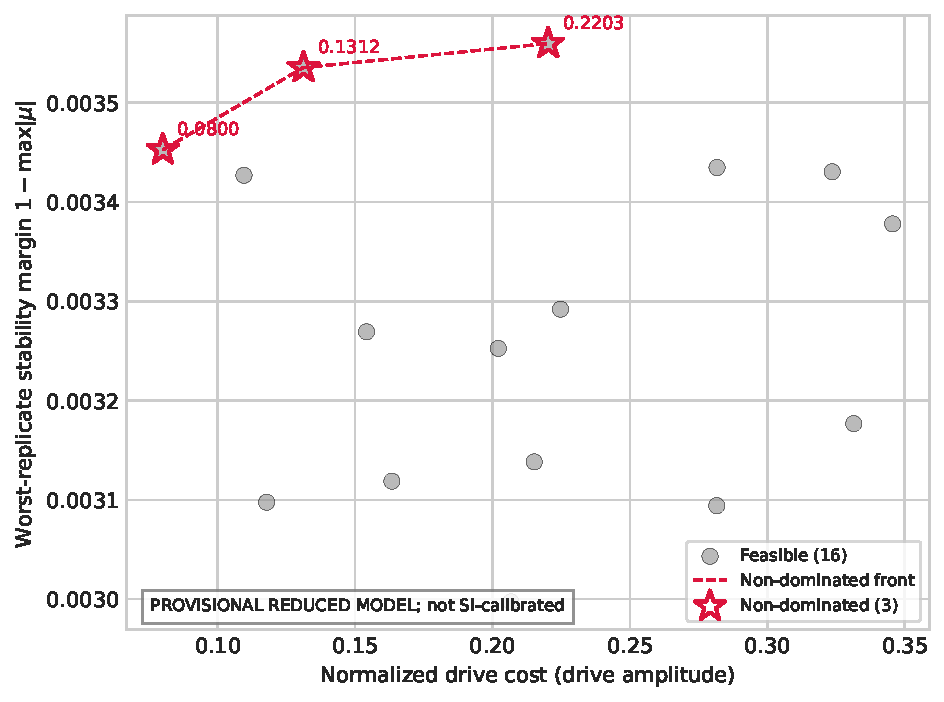
\includegraphics[width=0.72\textwidth,alt={Scatter of sixteen feasible candidates of the reduced adiabatic model in normalized drive cost versus worst-replicate stability margin, with the three non-dominated candidates marked by crimson stars and joined by a dashed front. The front trades increasing drive cost for increasing stability margin. Model-level only.}]{reduced_model_pareto_v4.pdf}
  \caption{Reduced-model (adiabatic) two-objective Pareto front. Sixteen feasible candidates (gray) in normalized drive cost versus worst-replicate stability margin $1-\max|\mu|$; the three non-dominated candidates (crimson stars, joined by the dashed front) are the points listed in \Cref{SI-tab:si-reduced-pareto}. Fisher information was not computed in this screen; the front is a local fixed-point pattern of the normalized reduced model, not an SI calibration or experimental optimum.}
  \label{SI-fig:si-reduced-pareto}
\end{figure}

\section{Amplitude-quadrature noise model cross-check}
\label{SI-sec:noise-model-crosscheck}

The measured record is $y=X_a+\nu_{\rm det}$ with $X_a=\Re(\alpha)$ the amplitude quadrature $(a+a^\dagger)/2$, whose vacuum variance is $1/4$. The Langevin diffusion coefficient that reproduces the quantum master equation for this quadrature is therefore $\kappa/4$ per amplitude quadrature, not $\kappa/2$ (the latter is the diffusion of the \emph{normalized} quadrature $(a+a^\dagger)/\sqrt2$, whose vacuum variance is $1/2$). We verified this normalization directly on the isolated optical sector of the reference point (the driven damped linear cavity, $g_1=g_2=0$): the truncated-Fock master equation~\cite{walls2008,gardiner1985} ($H=-\Delta a^\dagger a+E(a+a^\dagger)$, Lindblad $\sqrt{\kappa}\,a$) gives $\mathrm{Var}[(a+a^\dagger)/2]=\num{0.25}$, while the Langevin amplitude with noise $\kappa/2$ gives $\num{0.49}$ (a factor $2$ high) and with $\kappa/4$ gives $\num{0.245}$ (agreement below $\qty{2}{\percent}$). The mechanical thermal diffusion is correspondingly $\gamma_j(2n_{\rm th}+1)/4$ per amplitude quadrature. With these strengths the noise-only floor of the measured record is $\approx\num{0.25}$ and the strong-coupling observability ratios are $\num{7.6}$--$\num{17.0}\times$ the floor.

\section{Interpretation}
\label{SI-sec:interpretation}

The anchored set defines a \emph{reference} operating region, not a validated device calibration: $\omega_2$ is assumed near-degenerate with $\omega_m$ pending a two-resonator measurement, $J_m$ must be scanned rather than fixed, and the drive amplitude and detuning remain model-level coordinates. Any result computed at the anchored values therefore carries the same \emph{provisionally-calibrated} status as the reduced-model analysis of the main text and should not be presented as an experimental optimum.

Placing the strong-coupling hyperchaos regime against the anchors quantifies the reachability bound. The parameter-by-parameter comparison is reported once, in \Cref{SI-sec:feasibility-check} and \Cref{SI-tab:anchor-gap}: the couplings, the damping, and the cavity decay exceed their anchored values, the optomechanical coupling is the limiting coordinate, and the inter-resonator hopping $J_m/\omega_m=\num{0.08}$ lies within the Mathew scan range. The hyperchaos regime is therefore a model-level demonstration, not a prediction for the anchored device. The drive amplitude is not convertible to an input power without the pump frequency and external coupling, which neither anchor provides. The feasibility column of \Cref{SI-tab:si-pilot-vs-anchor} makes this judgment explicit per coordinate.

A feasibility frontier sharpens this bound. Because the radiation-pressure nonlinearity grows with the drive, the coupling at which hyperchaos first appears could in principle depend on the operating drive, so the single-point comparison above may misstate the true gap. Scanning the drive over $E\in[\num{0.5},\num{8.0}]$ and the coupling over $g_1/\omega_m\in[\num{0.02},\num{0.3}]$ (with $g_2=\num{0.9}g_1$), the full six-exponent spectrum shows that hyperchaos ($n_+\ge2$) occurs only at $E=\num{8}$, with an onset near $g_1/\omega_m\approx\num{0.14}$--$\num{0.18}$ (\Cref{SI-tab:si-feasibility-frontier}). Over this interval the second exponent is marginal and the order is seed-dependent ($n_+\in\{1,2\}$); the robust value $n_+=2$ for all three seeds begins at $g_1/\omega_m\approx\num{0.18}$, i.e. $\num{1525}\times$ the anchored $g_0/\omega_m=\num{1.18e-4}$. No drive retuning within the tested envelope lowers this onset, so the coupling gap is fundamental to the hyperchaos regime rather than an artefact of the single operating point above.

\begin{table}[h]
  \centering
  \caption{Feasibility frontier: the smallest optomechanical coupling at which the chaos ($n_+\ge1$) and hyperchaos ($n_+\ge2$) orders are reached, versus the drive $E$, from a log-spaced coupling grid $g_1/\omega_m\in[\num{0.02},\num{0.3}]$ with $g_2=\num{0.9}g_1$ and all other coordinates at the strong-coupling hyperchaos values above (the scan is taken at $\theta=\num{0}$). ``None'' means the order is not reached at any tested coupling. The $E=\num{8}$ hyperchaos cell reports the three-seed onset scan at $g_1\in[\num{0.14},\num{0.22}]$: the hyperchaos onset is a transition interval (second exponent marginal, seed-dependent $n_+\in\{1,2\}$, first appearance $\num{0.14}$); the robust onset (all three seeds) is $g_1/\omega_m\approx\num{0.18}$, i.e. $\num{1525}\times$ the anchored $g_0/\omega_m=\num{1.18e-4}$ (the coarse single-seed grid first reaches $n_+\ge2$ at $\num{0.203}$).}
  \label{SI-tab:si-feasibility-frontier}
  \begin{tabular}{@{}lcc@{}}
    \toprule
    $E$ & chaos onset $g_1/\omega_m$ & hyperchaos onset $g_1/\omega_m$ \\
    \midrule
    \num{0.5} & none & none \\
    \num{1.0} & none & none \\
    \num{2.0} & \num{0.203} & none \\
    \num{4.0} & \num{0.30} & none \\
    \num{8.0} & \num{0.094} & \num{0.14}--\num{0.18} (robust \num{0.18}) \\
    \bottomrule
  \end{tabular}
\end{table}

\section{Matched measurement Fisher on the chaotic attractor}
\label{SI-sec:attractor-fisher}

The matched force-sensing calculation of the main text is defined around a stable drive-locked orbit through its periodic covariance. On a chaotic attractor no stable orbit exists, so the same question is posed directly on the attractor: a weak external force on mechanical mode $1$, read out through $X_a=\Re(\alpha)$ under the same thermal, vacuum, and detector noise, with the classical measurement Fisher information evaluated from the ensemble-and-time mean and variance of the record and a central difference in the force (\num{1024} ensemble members, \num{120000} steps per configuration). On the attractor the record variance ranges from \num{1.9} to \num{4.3} at the tested points, of which the deterministic chaotic spread accounts for \num{1.8}--\num{4.1}; it is hundreds of times the detector-noise variance \num{0.01}, so the force-induced mean shift is resolved only where the spread is small enough relative to the sampling error. A derivative is reported only when it exceeds three bootstrap standard deviations of the record mean.

\Cref{SI-tab:si-attractor-fisher} lists the six tested configurations. At $E=\num{4}$ the flux-off record ($\theta=0$) gives $F_C=\num{1.08e-2}$ and the flux-on record ($\theta=\pi$) gives $F_C=\num{5.88e-3}$, a ratio \num{0.54}; the intermediate phase and all $E=\num{8}$ points fall below the resolution threshold and are not reported as finite gains. No flux-induced enhancement of the force-sensing Fisher information is therefore found on the chaotic attractor; where the comparison is resolved the flux phase reduces rather than raises $F_C$. The variance term carries \qty{71}{\percent}--\qty{89}{\percent} of $F_C$ in these cells (\qty{86}{\percent}--\qty{89}{\percent} at $E=\num{8}$), outside the lemma's sub-dominance premise, which holds on the stable orbit only. Per-cell detection floors (three bootstrap standard deviations) are $\num{1.4e-3}$, $\num{2.7e-3}$, $\num{8.1e-4}$ at $E=\num{4}$ and $\num{1.1e-3}$, $\num{2.0e-3}$, $\num{7.3e-4}$ at $E=\num{8}$. A \num{4096}-member rerun at $(E,\theta)=(4,\pi/2)$ still leaves the derivative below the three-standard-deviation mark ($|d|/\mathrm{SE}=\num{1.9}$), showing the sampling error is set by chaotic record variability rather than ensemble size. This is a classical measurement-Fisher calculation, not QFI, and it implies no chaotic-transduction sensing advantage.

\begin{table}[h]
  \centering
  \caption{Matched measurement Fisher information on the chaotic attractor at strong coupling. $\sigma^2_y$ is the record variance (dominated by the deterministic chaotic spread; the detector-noise variance is \num{0.01}); $\dd\langle y\rangle/\dd F$ is the central-difference response to the force; $F_C$ is the classical measurement Fisher information. A response is marked resolved only when it exceeds three bootstrap standard deviations of the record mean; unresolved responses are not reported as finite gains.}
  \label{SI-tab:si-attractor-fisher}
  \begin{tabular}{@{}cccccc@{}}
    \toprule
    $E$ & $\theta/\pi$ & $\sigma^2_y$ & $\dd\langle y\rangle/\dd F$ & $F_C$ & resolved \\
    \midrule
    \num{4} & 0 & \num{1.94} & \num{-0.071} & \num{1.08e-2} & yes \\
    \num{4} & 1/2 & \num{2.24} & \num{-0.045} & \multicolumn{1}{c}{---} & no \\
    \num{4} & 1 & \num{1.91} & \num{-0.056} & \num{5.88e-3} & yes \\
    \num{8} & 0 & \num{3.66} & \num{-0.016} & \multicolumn{1}{c}{---} & no \\
    \num{8} & 1/2 & \num{4.32} & \num{-0.018} & \multicolumn{1}{c}{---} & no \\
    \num{8} & 1 & \num{3.61} & \num{-0.022} & \multicolumn{1}{c}{---} & no \\
    \bottomrule
  \end{tabular}
\end{table}

\section{Semiclassical boundary of the strong-coupling classification}
\label{SI-sec:semiclassical-boundary}

The truncated-Fock master-equation cross-check of the main text validates the mean-field amplitude scale at the weakly coupled reference point, where the optical mode is a driven linear cavity whose coherent steady state is exact. At a strong-coupling chaotic point we extend this check to the optical sector: the truncated-Fock master equation for the cavity mode driven by the classical mechanical trajectories of the chaotic attractor ($E=\num{4.0}$, $\theta=0$, $n_+\in\{1,2\}$ over seeds and windows) converges toward $\langle a^\dagger a\rangle(t)=|\alpha(t)|^2$. The maximum relative deviation is $\num{4.6e-3}$ at $N_{\rm Fock}=\num{40}$ and $\num{6.6e-6}$ at $N_{\rm Fock}=\num{60}$. This is expected on general grounds---the optical Hamiltonian is linear in $a$---but it confirms that the optical factorization $\langle a^\dagger a\rangle\approx|\alpha|^2$ holds along the chaotic trajectory, not only at the stationary reference. At the weak-coupling reference the mean-field occupation $\langle|\alpha|^2\rangle=\num{0.032428}$ reproduces the single-mode truncated-Fock ($N_{\rm Fock}=\num{8}$) value $\num{0.032}$ to $\qty{1.3}{\percent}$. The time-averaged second-order correlation $g_2\approx\num{2.0}$ is super-Poissonian rather than coherent, as expected for a mixture of coherent amplitudes whose phase is modulated by the chaotic mechanical motion. At this trajectory the mean occupations are $\langle a^\dagger a\rangle=\num{6.121}$, $\langle b_1^\dagger b_1\rangle=\num{37.5}$, and $\langle b_2^\dagger b_2\rangle=\num{44.1}$. The standard relative quantum-fluctuation scale $1/\sqrt{\bar n}$ implied by these occupations is \qty{16}{\percent} ($\bar n=\num{37.5}$); at the hyperchaotic point below ($\bar n=\num{5e2}$) it shrinks to \qty{4}{\percent}. These are semiclassical scale estimates for the mechanical sector, not bounds on the Lyapunov spectrum or on quantum corrections to it. The mechanical sector is therefore in a high-occupation regime, but it remains semiclassical in the present calculation; no full two-mode quantum dynamics is claimed. The check does not solve the two-mechanical-mode quantum dynamics: the Lyapunov exponents characterize the mean-field dynamics rather than the quantum fluctuations, and no quantum observable (Wigner function, QFI) in the strong-coupling sector is computed in this study. This delimits the semiclassical treatment, now checked on the optical sector at a chaotic point and justified on the mechanical sector by its high occupation.

\paragraph{Hyperchaotic-point check.}
The same ladder is run at the hyperchaotic headline point ($E=\num{8.0}$, $\theta=\pi/2$). The maximum relative deviation of $\langle a^\dagger a\rangle$ from $|\alpha|^2$ is $\num{19.5}$, $\num{3.22}$, $\num{1.17e-3}$ and $\num{5.53e-7}$ at $N_{\rm Fock}=\num{20}$, $\num{40}$, $\num{60}$ and $\num{80}$: the $N_{\rm Fock}=\num{80}$ master equation tracks the mean-field occupation to $\num{5.53e-7}$ even on the hyperchaotic trajectory, where the mechanical motion drives the optical phase hardest. The occupations on the \num{2.0}-period analysis window are $\langle a^\dagger a\rangle=\num{6.9}$, $\langle b_1^\dagger b_1\rangle=\num{5.6e2}$, and $\langle b_2^\dagger b_2\rangle=\num{3.9e2}$ (bounded; a longer-transient probe at the same point---\num{400} drive periods of transient relaxation followed by a \num{200}-period measurement window---gives $\langle b_1^\dagger b_1\rangle=\num{3.96e2}$ and $\langle b_2^\dagger b_2\rangle=\num{4.04e2}$, so the mechanical occupations are quoted as scales of order $\num{4e2}$ rather than as window-precise means). A \num{1000000}-step Lyapunov re-check at the same point gives the spectrum $[\num{0.3245},\num{0.0482},\num{0.0154}, \num{-0.001},\dots]$, i.e.\ $n_+=3$ with the fourth exponent marginal at the threshold, consistent with the $n_+\in\{3,4\}$ spread of the strong-coupling map and the truncated-Wigner-approximation (TWA) ensemble at this point.

\paragraph{Truncated-Wigner robustness of the hyperchaos order.}
Because the mechanical occupations are large at the tested chaotic point ($\langle b_1^\dagger b_1\rangle=\num{37.5}$ and $\langle b_2^\dagger b_2\rangle=\num{44.1}$ in the master-equation cross-check), a full three-mode truncated-Fock master equation over the entire strong-coupling map is numerically out of reach: a Fock cutoff of order \num{100} on each mechanical mode (several times the mean occupation) and \num{20} on the optical mode requires a basis of order $(20\times100\times100)$ states, a density matrix of order \num{4e10} elements. The standard semiclassical-to-quantum bridge in this high-occupation regime is the truncated Wigner approximation, in which the quantum state is represented by an ensemble of classical trajectories with Wigner-sampled initial conditions and the c-number equations of motion coincide with the classical equations of the model. Quantum fluctuations therefore enter through the initial conditions with vacuum variance \num{0.5} per quadrature (an order-one fluctuation in $|\alpha|^2$). We recompute the full six-exponent spectrum from \num{12} Wigner-sampled initial conditions (variance \num{0.5} per coordinate) around each tested attractor and record the spread of the hyperchaos order $n_+$ (\Cref{SI-tab:si-twa}).

The bulk of the route persists across the tested ensemble. At $E=\num{8}$, $\theta=0$ the two positive exponents ($\num{3.5e-2}$ and $\num{2.5e-1}$) are separated from the largest negative exponent ($\num{-7.8e-3}$) by factors of $\num{4.5}$ and $\num{32}$, all \num{12} trajectories give $n_+=2$, and the leading exponent varies by only \qty{9}{\percent} across the ensemble. At the classification boundaries the order is threshold-conventional, as expected for a finite-time classification: at $E=\num{8}$, $\theta=\pi/2$ the TWA ensemble's nearest-to-threshold fourth exponent reaches $+\num{2.4e-3}$ (against $+\num{7.06e-4}$ for the production-map seed), only \num{2.4} times the positivity threshold \num{1e-3}, and the ensemble splits evenly between $n_+=3$ and $n_+=4$; at the chaos onset $E=\num{4}$, $\theta=0$ the second exponent is \num{1e-4} and the ensemble splits between $n_+=1$ and $n_+=2$. The ``up to four simultaneously unstable directions'' finite-time phrasing of the main text is therefore the correct level of claim: the hyperchaos route itself persists under quantum fluctuations at the TWA level, while the precise hyperchaos order at the extrema is threshold-conventional. This is a TWA-level check, not a full master-equation solution, and it supports no quantum-state (Wigner-negativity or QFI) claim.

\begin{table}[h]
  \centering
  \caption{Truncated-Wigner robustness of the finite-time hyperchaos order. For each strong-coupling point the full six-exponent spectrum is recomputed from \num{12} vacuum Wigner-sampled initial conditions (variance \num{0.5} per quadrature) around the attractor; $n_+^{\rm ref}$ is the deterministic reference order from the attractor-seeded reference trajectory (a different initial condition from the production-map seed: at $(8,\pi/2)$ it reads $4$ while the map seed reads $3$, both within the documented spread) and the ensemble column lists the spread of $n_+$ across the \num{12} trajectories. ``Nearest-to-threshold exponent'' is the Lyapunov exponent closest to the positivity threshold \num{1e-3}; its sign indicates whether it lies just above ($+$) or just below ($-$) the threshold, which governs the sensitivity of $n_+$ to finite fluctuations.}
  \label{SI-tab:si-twa}
  \small
  \setlength{\tabcolsep}{4pt}
  \begin{tabular}{@{}lcccc@{}}
    \toprule
    Point & $n_+^{\rm ref}$ & $n_+$ ensemble & Nearest-to-threshold & Leading exponent \\
    \midrule
    $E=\num{4}$, $\theta=0$ & $1$ & $1$--$2$ (8/4) & $+\num{1e-4}$ & \num{0.082}--\num{0.096} \\
    $E=\num{8}$, $\theta=0$ & $2$ & $2$ (12/12) & $-\num{7.8e-3}$ & \num{0.225}--\num{0.247} \\
    $E=\num{8}$, $\theta=\pi/2$ & $4$ & $3$--$4$ (6/6) & $+\num{2.4e-3}$ & \num{0.294}--\num{0.323} \\
    \bottomrule
  \end{tabular}
\end{table}

\section{Limitations and residual gaps of the consistency protocol}
\label{SI-sec:limitations}

The main text states four explicit residual gaps within its critical self-assessment; this section collects them in full so that the boundary of what the protocol certifies is explicit.

\paragraph{Gap 1: global structure of the chaotic attractor.}
The Floquet--Lyapunov protocol quantifies local instability rates around a converged drive-locked periodic orbit, and the matched-measurement Fisher protocol quantifies a \emph{local} information rate around the same orbit. Both deliver a consistent signature of the hyperchaos transition and of the matched gain, but neither characterizes the global basin structure of the chaotic attractor: uniqueness is not proved, and no basin-of-attraction calculation or multi-section Poincar\'e return map is performed here. The correlation-dimension estimate reported in the main text is a geometric consistency check of the sampled attractor ($D_2\le D_{\mathrm{KY}}$), not a characterization of the global basin structure. The $\num{432}/\num{432}$ classification ensemble and the $\num{180}/\num{180}$ full-map repeat reported in the main text reproduce the route across the declared finite ensembles, but the integer $n_+$ changes between neighbouring values for some seeds near marginal exponents, and the ensemble does not constrain \emph{which} physical initial condition feeds the observed chaotic set. A full basin and bifurcation-network analysis, beyond the present scope, would be required to draw a study-level uniqueness statement.

\paragraph{Gap 2: modest Fisher gain under realistic uncertainty.}
Even at the most favourable phase the matched force-sensing Fisher gain remains near unity (\num{1.32}$\times$ flux-off, \num{1.16}$\times$ single-mode), and the Monte-Carlo envelope on the uncalibrated hopping (log-uniform over $J_m/\omega_m\in[\num{1e-3},\num{1e-1}]$), thermal occupation (uniform over $n_{\mathrm{th}}\in[\num{0.01},\num{1.0}]$), and drive amplitude ({\raise.17ex\hbox{$\scriptstyle\pm$}}\qty{10}{\percent}) drags the median to \num{1.039}$\times$ (production ensemble; \num{1.056}--\num{1.060} across three replicate ensembles, pooled-\num{240} median \num{1.050}; \qty{90}{\percent} CI $[1.025,\,1.053]$ within-ensemble) against the flux-off reference, and to \num{1.019}$\times$ (replicates \num{1.028}--\num{1.030}, pooled median \num{1.025}; CI $[\num{1.012},\num{1.026}]$) against the single-mode reference. On the chaotic attractor the same protocol returns a null result, so the gain can be reported as a \emph{protocol-level} demonstration without being claimed as a quantum sensing advantage: the observation time is one drive period and the model is linear-detuning-limited. The numerical gain is consistent with the matched reference (\Cref{SI-sec:matched-fisher}) and is reported here as such, not as a sensing breakthrough.

\paragraph{Gap 3: validity boundary of the mean-field protocol.}
The truncated-Fock master equation cross-checks the mean field to \qty{1.3}{\percent} at the weak-coupling reference and to a maximum relative occupation deviation of $\num{6.6e-6}$ at $N_{\rm Fock}=\num{60}$ for the chaotic point ($E=\num{4}$), and $\num{5.53e-7}$ at $N_{\rm Fock}=\num{80}$ ($\num{1.17e-3}$ at $N_{\rm Fock}=\num{60}$) for the hyperchaotic point ($E=\num{8}$) (\Cref{SI-sec:semiclassical-boundary}); the truncated-Wigner trajectory ensemble reproduces the deterministic order $n_+\!=\!2$ in twelve of twelve sampled trajectories at ($E=\num{8}$, $\theta=0$) (\Cref{SI-tab:si-twa}). Both checks support use of the mean field for the qualitative route described in the main text (bifurcation sequence, finite-time hyperchaos order, matched gain), but neither extends to a fully quantum reconstruction or a quantum sensing claim. In particular, the master-equation truncation (cross-checked at $N_{\rm Fock}\!=\!8$ at the weak-coupling reference and converged at $N_{\rm Fock}\!=\!60$ for the chaotic point and $N_{\rm Fock}\!=\!80$ for the hyperchaotic point) is sufficient for the present dynamical regimes but does not span the deep strong-coupling sector needed for a sustained quantum-state claim.

The protocol therefore establishes a coherent-model dynamical repertoire (Floquet--Lyapunov consistency, hyperchaos route, matched Fisher null on the attractor) and includes a quantum cross-check \emph{at the levels just stated}. Claims outside those levels---basin uniqueness, calibrated sensing advantage, full-state quantum reconstruction---are explicitly not made. The two experimental steps identified in the Outlook of the main text ($\omega_2$ ultrasound calibration; a multi-gigahertz mechanical-mode platform) would close the calibration side of gap 2 and provide the parameter fidelity required for gap 3 to be addressed in a fully quantum manner.

\section{Strong-coupling sector feasibility check}
\label{SI-sec:feasibility-check}

The Discussion in the main text anchors the hyperchaotic regime to the $\num{2542}\times$ silicon optomechanical platform of Mayor \emph{et al.} (2025). This section reports the same comparison parameter-by-parameter, so the order-of-magnitude gap is verifiable rather than asserted.

The physically anchored reference set (\Cref{SI-sec:anchor}) supplies the device-level numbers: $\omega_m/2\pi=\qty{7.436}{\giga\hertz}$, $g_{\rm anchor}/\omega_m\!\approx\!\num{1.18e-4}$, $\gamma_{\rm anchor}/\omega_m\!\approx\!\num{2.78e-5}$, and $\kappa_{\rm anchor}/\omega_m\!\approx\!\num{0.108}$. The strong-coupling sector of the present manuscript uses $(g_1,g_2)/\omega_m\!=\!(\num{0.30},\num{0.27})$, $\gamma_{1,2}/\omega_m\!=\!\num{0.02}$, and $\kappa/\omega_m\!=\!1$. The matching factor (defined as the dimensionless ratio of the present parameter over the anchored parameter) is reported per parameter in \Cref{SI-tab:anchor-gap}.

\begin{table}[h]
  \centering
  \caption{Matching factor of the strong-coupling sector relative to the silicon-optomechanical anchor of Mayor \emph{et al.}~(2025). The factor is the dimensionless ratio of the dimensioned parameter used in the present work divided by the same parameter inferred from the anchored platform. Every factor lies above unity by at least one order of magnitude; the hyperchaotic regime is therefore a model-level extension, not a calibrated device prediction. The $J_m/\omega_m$ anchor entry spans the scan range of the Mathew \emph{et al.}~feasibility study.}
  \label{SI-tab:anchor-gap}
  \begin{tabular}{@{}lcc@{}}
    \toprule
    Parameter (dimensionless ratio) & Present sector & Mayor \emph{et al.}~anchor \\
    \midrule
    $g_1/\omega_m$ & \num{0.300} & \num{1.18e-4} \\
    $g_2/\omega_m$ & \num{0.270} & \num{1.18e-4} \\
    $\gamma/\omega_m$ & \num{0.020} & \num{2.78e-5} \\
    $\kappa/\omega_m$ & \num{1.000} & \num{0.108} \\
    $J_m/\omega_m$ & \num{0.080} & $[\num{1e-3},\num{1e-1}]$ \\
    \bottomrule
  \end{tabular}
\end{table}

\paragraph{Interpretation.}
The matching factor ranges from $\num{9.3}\times$ ($\kappa$) to $\num{2542}\times$ ($g_1$, three orders of magnitude above the resolved-sideband single-photon coupling). The $\num{2542}\times$ headline-sector factor is evaluated at the mapped strong-coupling point ($g_1/\omega_m=\num{0.30}$); the feasibility-frontier scan places the robust hyperchaos onset lower, at $g_1/\omega_m\approx\num{0.18}$, i.e.\ $\num{1525}\times$ the anchor (\Cref{SI-tab:si-feasibility-frontier}). The hyperchaotic regime is therefore not demonstrated by the anchored silicon optomechanical platform; broader near-term platform feasibility is not established by this comparison. The main text states the regime as a model-level demonstration, and the present table makes the per-parameter basis of that statement explicit.

\section{Initial-condition robustness of the long-window sweep}
\label{SI-sec:initial-condition-robustness}

The $\num{180}/\num{180}$ full-map repeat (three seeds at twelve phases and five drives) reported in the main text tests the reproducibility of the positive-exponent classification across the declared finite ensemble (see \Cref{MAIN-fig:hyperchaos-map}). It does not establish global attractor uniqueness or asymptotic convergence. This section documents the dependence of the classification on the initial-condition family through the classification ensemble (twelve seeds at twelve phases and three drives); the three-seed repeat of the complete map is reported in \Cref{SI-sec:convergence}, so both cross-checks are documented in full.

\paragraph{Classification ensemble: twelve seeds, twelve phases, three drives.}
The map was extended to twelve independent seeds at each of twelve flux phases and three drives: \num{432} long-window records of \num{1000000} steps (transient \num{100000}), $\num{432}/\num{432}$ completed at the positivity threshold \num{1e-3}. \Cref{SI-tab:si-twelve-seed} gives the seed range of $n_{+}$ at every phase. Initial conditions are drawn i.i.d.\ $\mathcal{N}(0,0.1^2I_6)$ (six-dimensional, $\sigma=\num{0.1}$ per component) from \texttt{default\_rng(seed)}: map seeds run $20260815+di\cdot12+ti$ and the robustness ensemble uses contiguous per-drive seed blocks, \num{432} unique seeds in all; the flank and second-coupling maps restart the same rule from base \num{20271001} and \num{20270901} respectively; every record stores its seed. The onset at $E=\num{1}$ is phase-locked: $n_{+}=1$ at $\theta=\pm2\pi/3$ for all \num{12} seeds, while every other phase gives $n_{+}=0$ (except two seeds at $\theta=-5\pi/6$). At $E=\num{4}$ the count is seed-dependent at $\theta=0$ ($n_+\in\{1,2\}$, the marginal second exponent) and robustly $1$ at $|\theta|=\pi$. At $E=\num{8}$ the count is unanimously $n_{+}=2$ for all \num{12} seeds at eight of the twelve phases, and $n_{+}\in\{3,4\}$ at $\theta=\pm\pi/3$ and $\theta=+\pi/2$; at $\theta=-\pi/2$ the spread is $n_+\in\{2,3,4\}$. The seed-to-seed spread is at most one at eleven of twelve phases (the exception being that $\theta=-\pi/2$). The integer ranges agree at $\theta$ and $-\theta$ at all but two of the fifteen mirrored phase pairs ($E=\num{1}$, $\theta=\mp5\pi/6$ and $E=\num{8}$, $\theta=\mp\pi/2$), supporting the phase-modulation statement but, as before, not establishing exact $\theta\to-\theta$ symmetry, and they do not constitute a global uniqueness proof: the ensemble is larger by a factor of four per point, not infinite. A second full twelve-phase, five-drive map at reduced coupling ($g_1/\omega_m=\num{0.2}$, $g_2/\omega_m=\num{0.18}$) shows the same flux modulation with a lowered ceiling: $n_+$ spans $\{1,2\}$ at $E=\num{2.0}$, $\{0,2\}$ at $E=\num{4.0}$ and $\{1,3\}$ at $E=\num{8.0}$, peaking near $\theta=\pm\pi/3$ against a flux-off baseline of $2$.

\begin{table}[h]
  \centering
  \caption{Second-coupling map ($g_1/\omega_m=\num{0.2}$, $g_2/\omega_m=\num{0.18}$): $n_{+}$ range over twelve phases per drive (\num{1e6} steps; seeds \num{20270901}--\num{20270960}).}
  \label{SI-tab:si-second-coupling}
  \begin{tabular}{@{}ll@{}}
    \toprule
    $E$ & $n_{+}$ range (12 phases) \\
    \midrule
    \num{0.2} & \num{0} \\
    \num{1.0} & \num{0} \\
    \num{2.0} & $\{1,2\}$ \\
    \num{4.0} & $\{0,2\}$ \\
    \num{8.0} & $\{1,3\}$, peaking near $\theta=\pm\pi/3$ \\
    \bottomrule
  \end{tabular}
\end{table}

\begin{table}[h]
  \centering
  \caption{Seed range of the hyperchaos order $n_{+}$ over \num{12} seeds at each of twelve flux phases and three drives (threshold \num{1e-3}, \num{1e6} steps; $\num{432}/\num{432}$ completed). ``Range'' is min--max over the \num{12} seeds at that phase; the $-\pi$ and $+\pi$ grid ends are identified.}
  \label{SI-tab:si-twelve-seed}
  \small
  \begin{tabular}{@{}lccc@{}}
    \toprule
    $\theta/\pi$ & $E=1$ & $E=4$ & $E=8$ \\
    \midrule
    $-1$    & $0$   & $1$   & $2$   \\
    $-5/6$  & $0$--$1$ & $1$   & $2$   \\
    $-2/3$  & $1$   & $1$--$2$ & $2$   \\
    $-1/2$  & $0$   & $2$--$3$ & $2$--$4$ \\
    $-1/3$  & $0$   & $2$--$3$ & $3$--$4$ \\
    $-1/6$  & $0$   & $2$   & $2$   \\
    $0$     & $0$   & $1$--$2$ & $2$   \\
    $+1/6$  & $0$   & $2$   & $2$   \\
    $+1/3$  & $0$   & $2$--$3$ & $3$--$4$ \\
    $+1/2$  & $0$   & $2$--$3$ & $3$--$4$ \\
    $+2/3$  & $1$   & $1$--$2$ & $2$   \\
    $+5/6$  & $0$   & $1$   & $2$   \\
    \bottomrule
  \end{tabular}
\end{table}

\section{Local susceptibility--stretching covariation on the attractor}
\label{SI-sec:local-fisher-stretching}

The main text explains the null matched-Fisher gain on the chaotic attractor with the matched-Fisher lemma: signal and noise projected onto the unstable manifold share the same stretching. This section tests that explanation directly on the trajectory, at the window scale, instead of only through the time-averaged statistic.

\paragraph{Method.}
At six drive--phase points ($E\in\{4,8\}$, $\theta/\pi\in\{0,1/2,1\}$) one trajectory of \num{1000000} steps (transient \num{100000}) is integrated with the same fixed-step RK4/QR backend as the production map. Alongside the state, the force-response vector $w'=J(x)\,w+e_{F}$, $e_{F}=(0,0,0,1,0,0)$ (a constant weak force on the $\beta_{1}$ momentum equation), is integrated with $w$ reset to zero at every window boundary of \num{2000} steps (\num{20} time units). This is the exact window-restricted linear response $S_{k}=\partial_{F}\langle X_{a}\rangle$ over window $k$, with no finite-difference nonlinearity. Per window the integration also records the local finite-time Lyapunov exponents $\lambda_{k}$ (QR block accumulators over the same window) and the local record spread $\sigma_{k}$ (standard deviation of $X_{a}=\operatorname{Re}\alpha$ within the window). The window-resolved Fisher proxy is $f_{k}=S_{k}^{2}/\sigma_{k}^{2}$. Each point contributes \num{450} windows, and all six points return finite records with positive $\sigma_k$ and $|S_k|$.

\paragraph{Shared stretching.}
Signal and noise both co-vary positively with the same local stretching at every point (\Cref{SI-tab:si-local-fisher} and \Cref{SI-fig:si-local-fisher}): $\rho(\lambda_{k},|S_{k}|)$ ranges from $+0.371$ to $+0.639$ and $\rho(\lambda_{k},\sigma_{k})$ from $+0.104$ to $+0.569$ (Spearman, \num{450} windows per point). This is the window-scale signature of the lemma's premise: the same local Lyapunov exponent that stretches the trajectory also controls both the force response and the record spread.

The two responses are not equal, however. The log-log slopes against $\lambda_{k}$ are $7.5$--$13.1$ for $\ln|S_{k}|$ but only $0.12$--$0.58$ for $\ln\sigma_{k}$: within a \num{20}-time-unit window the record spread saturates at the attractor scale while the force response keeps accumulating. The local proxy is therefore not flat---it grows with local stretching ($\rho(\lambda_{k},\ln f_{k})=+0.37$ to $+0.63$, coefficient of variation \num{6.5}--\num{13.7}). This asymmetry is a new nuance of the budget picture and is reported rather than suppressed: the matched-Fisher lemma concerns the time-averaged, matched-resource statistic, whereas the local proxy here is a window-restricted diagnostic.

\paragraph{Flux-phase dependence of the local budget.}
Two-sample Kolmogorov--Smirnov tests on the window distributions of $\ln f_{k}$ (\num{450} windows per phase) give the local counterpart of the global null result. At $E=\num{4}$, where the global matched Fisher resolves both $\theta=0$ and $\theta=\pi$, the proxy is statistically indistinguishable between $\theta=0$ and $\theta=\pi/2$ ($p=0.205$) and its median is \emph{lower} at $\theta=\pi$ than at $\theta=0$ ($p=0.012$): no flux phase supplies a local enhancement mechanism, and the direction matches the resolved global ratio $F_C(\pi)/F_C(0)=0.54$ (\cref{SI-sec:attractor-fisher}). At $E=\num{8}$ the $\theta=0$ and $\theta=\pi$ distributions are statistically indistinguishable ($p=0.766$), consistent with the global statistic being below resolution at that drive. The intermediate phase $\theta=\pi/2$ differs from $\theta=\pi$ at both drives and from $\theta=0$ at $E=\num{8}$ ($p\le\num{1e-5}$); the global Fisher at that phase is likewise below resolution, so the local difference cannot be converted into a global gain claim either way. These are descriptive, model-level, classical linear-response statements on the tested trajectories; no quantum, SQL, or device claim follows from them. Window-to-window lag-1 autocorrelation of $\ln f_k$ is $\num{-0.06}$--$\num{+0.13}$ (effective $N$ $\num{347}$--$\num{504}$ vs nominal $\num{450}$), leaving the reported $p$-values essentially unchanged; the three rejections survive Holm at $\alpha=\num{0.05}$ over the five cross-phase comparisons.

\begin{table}[h]
  \centering
  \caption{Window-resolved covariation at the six tested points. $\rho$ is the Spearman correlation over \num{450} windows; the slopes are ordinary least-squares fits of the log-log response against the local finite-time Lyapunov exponent $\lambda_{k}$.}
  \label{SI-tab:si-local-fisher}
  \small
  \begin{tabular}{@{}llrrrr@{}}
    \toprule
    Point & Windows & $\rho(\lambda_k,|S_k|)$ & $\rho(\lambda_k,\sigma_k)$ & $\mathrm{d}\ln|S|/\mathrm{d}\lambda$ & $\mathrm{d}\ln\sigma/\mathrm{d}\lambda$ \\
    \midrule
    $E=\num{4}$, $\theta=0$ & \num{450} & $\num{+0.440}$ & $\num{+0.104}$ & $\num{7.5}$ & $\num{0.12}$ \\
    $E=\num{4}$, $\theta=\pi/2$ & \num{450} & $\num{+0.475}$ & $\num{+0.389}$ & $\num{10.1}$ & $\num{0.55}$ \\
    $E=\num{4}$, $\theta=\pi$ & \num{450} & $\num{+0.371}$ & $\num{+0.116}$ & $\num{8.4}$ & $\num{0.18}$ \\
    $E=\num{8}$, $\theta=0$ & \num{450} & $\num{+0.630}$ & $\num{+0.569}$ & $\num{10.3}$ & $\num{0.58}$ \\
    $E=\num{8}$, $\theta=\pi/2$ & \num{450} & $\num{+0.639}$ & $\num{+0.245}$ & $\num{13.1}$ & $\num{0.25}$ \\
    $E=\num{8}$, $\theta=\pi$ & \num{450} & $\num{+0.583}$ & $\num{+0.383}$ & $\num{10.5}$ & $\num{0.34}$ \\
    \bottomrule
  \end{tabular}
\end{table}

\begin{figure}[h]
  \centering
  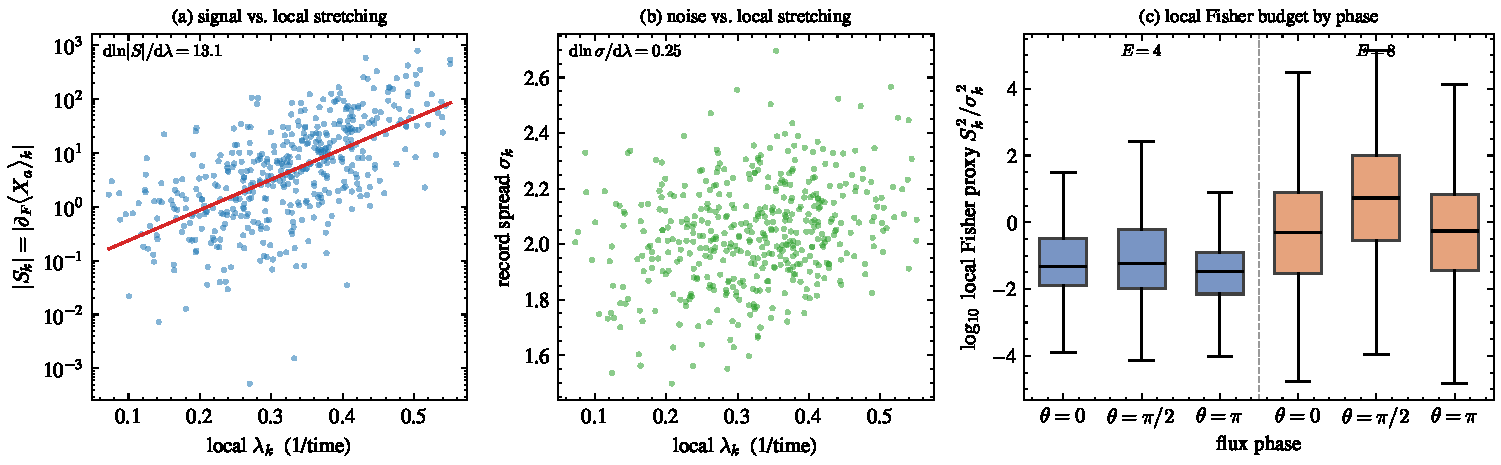
\includegraphics[width=\textwidth,alt={Three panels of the window-resolved local analysis. (a) The local force-to-observable susceptibility against the local finite-time Lyapunov exponent at E=8, theta=pi/2 shows a strong positive trend with fitted slope d ln|S|/d lambda = 13.1. (b) The local record spread against the same exponent is nearly flat with slope 0.25. (c) Grouped box plots of the log local Fisher proxy for all six drive and flux-phase points, split by drive. Model-level linear response only.}]{local_fisher_stretching.pdf}
  \caption{Window-resolved susceptibility--stretching covariation on the chaotic attractor at \num{450} windows per point. (a)~Local force-to-observable susceptibility $|S_{k}|$ against the local finite-time Lyapunov exponent at $E=\num{8}$, $\theta=\pi/2$: the signal responds strongly to local stretching. (b)~Local record spread $\sigma_{k}$ against the same exponent: the noise response is nearly flat because the within-window spread saturates at the attractor scale. (c)~Distribution of the local Fisher proxy $S_{k}^{2}/\sigma_{k}^{2}$ (logarithm) at all six drive--phase points. Model-level classical linear response only.}
  \label{SI-fig:si-local-fisher}
\end{figure}

\bibliography{Chaos_Floquet_SyntheticFlux}

\end{document}